
\begin{center}
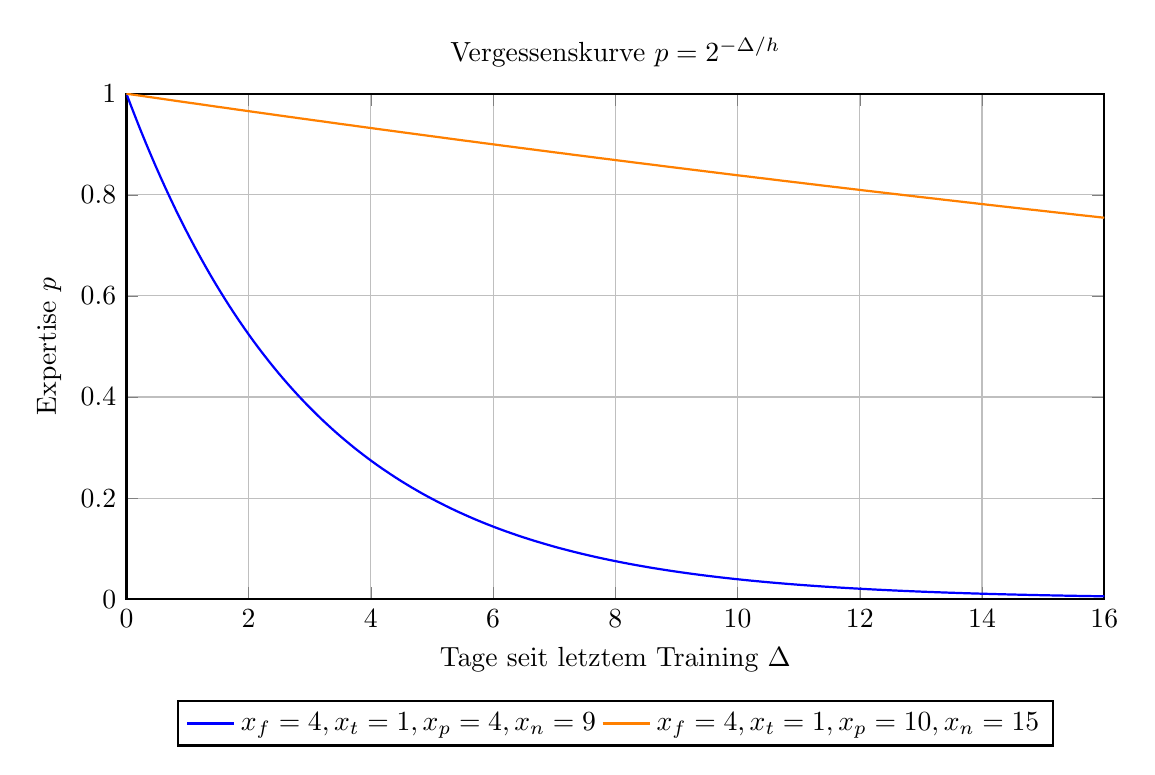
\begin{tikzpicture}
\begin{axis}[
    width=14cm,
    height=8cm,
    xlabel={Tage seit letztem Training $\Delta$},
    ylabel={Expertise $p$},
    xmin=0, xmax=16,
    ymin=0, ymax=1,
    samples=200,
    grid=major,
    thick,
    domain=0:16,
    legend style={at={(0.5,-0.2)}, anchor=north, legend columns=-1},
    title={Vergessenskurve $p = 2^{-\Delta / h}$}
]

% Parameter
\def\xf{4}
\def\xt{1}
\def\xp{4}
\def\xn{\xf+\xt+\xp}
\def\thetaf{-0.6}
\def\thetat{0.2}
\def\thetap{0.6}
\def\thetan{0.1}

% Berechnung der Halbwertszeit
\pgfmathsetmacro{\h}{
  2^((\thetaf)*(\xf) + (\thetat)*(\xt) + (\thetap)*(\xp) + (\thetan)*(\xn))
}
\pgfmathsetmacro{\g}{
  2^((\thetaf)*(\xf) + (\thetat)*(\xt) + (\thetap)*(10) + (\thetan)*(15))
}

% Plot der Vergessenskurve
\addplot[
    blue,
    thick
]
{2^(-x / \h)};
\addlegendentry{$x_f=\pgfmathprintnumber{\xf}, x_t=\pgfmathprintnumber{\xt}, x_p=\pgfmathprintnumber{\xp}, x_n=9$}

\addplot[
    orange,
    thick
]
{2^(-x / \g)};
\addlegendentry{$x_f=\pgfmathprintnumber{\xf}, x_t=\pgfmathprintnumber{\xt}, x_p=10, x_n=15$}

%\addlegendentry{$h = \pgfmathprintnumber[fixed, precision=2]{\h}$}

\end{axis}
\end{tikzpicture}
\end{center}
